\documentclass[twocolumn, 9pt]{jsproceedings}

\interfootnotelinepenalty=10000

\title{Weightless Neural Networks for Depth Map Estimation}

\author{Helio Perroni Filho (Doctorate Course, 1st year)\authorrefmark{1}}

\affiliation{Intelligent Robotics Laboratory, OHYA's group}

\abstract{
ZETA is a Weightless Neural Network (WNN) for monocular depth map estimation. Weightless Neural Networks mirror an alternative view on how biological neurons work. As a machine learning tool, they are remarkable for both its simplicity and flexibility, being applicable to a wide range of classification problems. This article describes the class of Weightless Neurons used in ZETA -- known as Virtual Generalizing Random Access Memory (VG-RAM) neurons -- as well as the system's overall architecture. Its accuracy is reported, and directions for future improvements are discussed in the conclusion.
}

\keywords{Machine Learning, Sensing, Image Processing}

\begin{document}
\thispagestyle{myheadings}
\markright{2013年度 第2回 山彦シンポジウム [2013/11/30--12/1 つくば国際会議場]}
\maketitle

\authorreftext{1}{Graduate School of Systems and Information Engineering,\\ University of Tsukuba}

\section{Introduction}

Even among machine learning researchers, the term ``neural network'' has become virtually synonymous with ``perceptron'' -- or more specifically, Frank Rosenblatt's multilayer perceptron model~\cite{rosenblatt58}. A perceptron neuron \(P\) can be described as a tuple:
\begin{equation*}
P = (\Phi , B , W) \quad B \in \mathbb{R} \; , \; W \in \mathbb{R}^n
\end{equation*}

Where \(\Phi\) is the activation function (generally the {\it sigmoid} or {\it hyperbolic tangent} function), \(B\) the neuron's bias and \(W\) the vector of synaptic connection weights. The neuron's response to an input vector \(X\) is described as:
\begin{equation*}
P (X) = \Phi(B + \sum_{k = 1}^{n} {x_k w_k}) \; , \; X \in \mathbb{R}^n
\end{equation*}

Figure~\ref{fig:perceptron} presents these concepts in an schematic diagram.

\begin{figure}[h!]
\includegraphics[width=\columnwidth]{perceptron.pdf}
\caption{Schematic diagram of a single neuron in a multilayer perceptron network. The dot product of input and weight vectors \(X\) and \(W\) is added to bias \(B\); the result is fed to activation function \(\Phi\), giving off neuron output \(Y\).}
\label{fig:perceptron}
\end{figure}

Perceptron neurons are related to the rate coding model often attributed to Edgar Adrian~\cite{adrian26}. According to this theory, biological neurons communicate in an analog protocol, where information is encoded as the rate of electrochemical reactions or {\it spikes} an excited neuron gives off over a period of time. This, however, is not the only standing theory on how living neurons work. In the alternative sparse coding model, the neural communication protocol is digital: individual neurons are restricted to single-bit outputs (whether they give off a spike or not), and information is encoded as the set of which neurons are ``spiking'' at a given moment~\cite{olshausen04}.

\begin{figure}[h!]
\includegraphics[width=\columnwidth]{weightless.pdf}
\caption{Abstract diagram of a single neuron in a weightless neural network. An input, consisted by a string of single-bit values, is used to address a {\it content-addressable memory}, retrieving an stored value that is taken as the neuron's output.}
\label{fig:weightless}
\end{figure}

{\it Weightless neurons} can be thought of as the computing counterpart of the sparse coding model for biological neurons. Instead of real-valued vectors, they accept strings of single bits as inputs; these inputs are used to address some sort of {\it content-addressable memory}, retrieving an stored value that is taken as the neuron's output. Several variations of this basic design -- illustrated in Figure~\ref{fig:weightless} -- have been developed over the years, such as the RAM node, Probabilistic Logical Node (PLN), Goal Seeking Neuron (GSN) and Virtual Generalizing Random Access Memory (VG-RAM)~\cite{ludermir98}. This last variant is unique in that, while inputs are still required to be bit strings, outputs are not so restricted, and can be of any desired type~\cite{souza08}.

This article presents a primer on VG-RAM weightless neural networks. First an original notation is introduced, largely based on the conventions from set-builder notation, supplemented with concepts from Bird's Theory of Lists~\cite{bird87}. A theoretical framework is constructed to enable reasoning on VG-RAM networks in purely abstract terms; to the author's knowledge, this is the first time such an endeavor has been attempted. The article then turns to the problem of depth map estimation for single monocular images as a use case for VG-RAM WNN's. A procedure for representing images as bit strings for neuron training is designed, and the network's architecture is defined. The resulting ZETA system is tested against a database of images and corresponding depth maps; its performance is contrasted to that of estimators based on {\it Markov Random Fields}, which currently present the best known results. The article concludes by discussing directions for further research and possible improvements to the current system.

\section{Overview of VG-RAM WNN's}

A VG-RAM weightless neuron stores both a list of {\it known inputs} encoded as {\it bit strings}, and an associated list of {\it outputs} from an arbitrary set. During training, input / output pairs are written directly to the neuron's memory. When an input bit string is presented to the trained neuron, it returns the output associated to the best matching known input.

A VG-RAM neuron \(R\) can thus be described as a tuple:
\begin{equation}
R = (r, I, O)
\end{equation}

Where \(I\) is the list of known inputs, and \(O\) the list of associated outputs:
\begin{alignat}{10}
I & = [i_1 , & i_2 , & \dotsc , i_k , & \dotsc , i_n & ] \\
O & = [o_1 , & o_2 , & \dotsc , o_k , & \dotsc , o_n & ]
\end{alignat}

As mentioned previously, outputs can be of any type, but inputs must be bit strings of some fixed length \(r\):
\begin{equation*}
i_k = [ b_1 , b_2 , \dotsc , b_k , \dotsc , b_r ] \; | \; b_k \in \mathbb{B} = \{ 0 , 1 \}
\end{equation*}

Or in a more compact notation:
\begin{equation}
i_k \in \mathbb{B}^r
\end{equation}

The indexing operation \([\cdot]\) describes read and write access to VG-RAM neural memory, so that for an input \(b \in \mathbb{B}^r\) and output \(y\):
\begin{equation}
R[b] = y \quad \equiv \quad R = (r, I \cup [b], O \cup [y])
\end{equation}
\begin{equation}
y = R[b] \quad \equiv \quad y = o_k \in O \; | \; i_k = \arg \min_{i \in I} { \; d ( b , i ) }
\end{equation}

Where the concatenation operation \(\cup\) is defined for lists such that \([a, b] \cup [c] = [a, b, c]\), and the {\it bitwise distance} \(d\) between bit strings is defined as:
\begin{equation}
d ( i_a , i_b ) = \sum_{k = 1}^{r} {| i_a[k] - i_b[k] |}
\end{equation}

Training a VG-RAM neuron, as definition (5) makes clear, is just a matter of appending input / output pairs to its internal memory. Therefore, a neuron can be completely trained by a single pass through a training data set, in time linearly proportional to the size of the set.

Furthermore, definitions (6) and (7) show that VG-RAM neurons perform a {\it nearest-neighbor search} over the list \(I\) of known bit strings. Given an unknown bit string \(b\), it is expected that the response \(o_k\) associated to the closest known input \(i_k\) will represent a ``good enough'' approximation of \(b\)'s unknown ``true'' output \(y\); obviously, whether this is true depends entirely on the quality of the training data. The process is illustrated in Figure~\ref{fig:vg-ram}.

\begin{figure}[h!]
\includegraphics[width=\columnwidth]{vg-ram.pdf}
\caption{Query processing in a VG-RAM neuron containing three known input bit strings of length \(3\). The distances between the input bit string \(b\) and the three known inputs \(i_1\), \(i_2\) and \(i_3\) are calculated, and the output (\(o_2\)) associated to the closest known input (\(i_2\)) is returned.}
\label{fig:vg-ram}
\end{figure}

In principle, VG-RAM neurons could approximate a function from a domain set \(X\) to an image set \(Y\), regardless of how they are related, as long as there exists a function \(f : X \to \mathbb{B}^r \) mapping elements from \(X\) to bit strings of finite length \(r\). This would imply that {\it any} data structure of a constant or bounded size -- images, sound clips, database records, etc. -- could directly index a VG-RAM neuron, simply by taking its binary representation as a bit string.

In practice, however, such a ``black box'' approach is very unlikely to succeed. The problem is that the points in the metric space \((\mathbb{B}^r , d)\) lie at the edges of the unit hypercube of of dimension \(r\). When \(r\) increases, the number of distinct elements that can be represented grows, but so does the complexity of the space: as shown in Figure~\ref{fig:hypercube}, this quickly leads to an explosion in the number of close relationships between inputs. As a result, bitwise distance between binary representations of complex objects will rarely correlate well to any subjective or domain-defined measure of similarity.

\begin{figure}[h!]
\includegraphics[width=\columnwidth]{hypercube.pdf}
\caption{Petrie polygons of the unit hypercube in 3 (a), 4 (b) and 8 (c) dimensions.}
\label{fig:hypercube}
\end{figure}

Increasing \(r\) also affects computing resource usage: not only storage requirements increase with the length of bit strings, but so does the time spent searching among them. Using a naive search algorithm, discovering the known input \(i_k\) which is closest to \(b\) takes \(\theta(r|I|)\). Therefore, VG-RAM neurons are vulnerable to the {\it curse of dimensionality} -- as the dimension of \(\mathbb{B}^r\) increases,  amassing and sifting through sufficient numbers of bit strings soon becomes impractical.

In order to design efficient mapping functions and mitigate the curse of dimensionality, it's necessary to explore the structural properties and inherent relationships between the domain and image sets. Assuming elements from \(X\) and \(Y\) are not monolithic, but can be broken down into lists of {\it features} from respective {\it feature sets} \(F\) and \(G\):
\begin{equation}
x_k = [ f_{k,1} , \dotsc , f_{k,v} , \dotsc , f_{k,m} ] \quad x_k \in X \;\; , \;\; f_{k,v} \in F
\end{equation}
\begin{equation}
y_k = [ g_{k,1} , \dotsc , g_{k,v} , \dotsc , g_{k,m} ] \quad y_k \in Y \;\; , \;\; g_{k,v} \in G
\end{equation}

Given a training set \(T\):
\begin{equation}
T = [ (x_1 , y_1), \dotsc, (x_k , y_k), \dotsc, (x_n , y_n) ]
\end{equation}

The relationship implied by \((x_k , y_k)\) can be reasonably expected to be a function of the features present in each element. This can be modeled as a set of functions:
\begin{equation}
P = \{ p_1 , \dotsc , p_v , \dotsc , p_m \}
\end{equation}

Where each function \(p_v\) approximates feature \(g_{k,v}\) of \(y_k\) from a {\it feature subset} \(x'_{k,v}\) of \(x_k\):
\begin{equation}
g_{k,v} \approx p_v(x'_{k,v}) \quad x'_{k,v} \subseteq x_k \; , \; g_{k,v} \in y_k
\end{equation}

The training set can likewise be disassembled into a number of {\it feature training sets}:
\begin{align}
& T_1 = [ (x'_{1,1} , g_{1,1}), \dotsc, (x'_{n,1} , g_{n,1}) ] \\
& T_2 = [ (x'_{1,2} , g_{1,2}), \dotsc, (x'_{n,2} , g_{n,2}) ] \notag\\
& \dots \notag\\
& T_v = [ (x'_{1,v} , g_{1,v}), \dotsc, (x'_{n,v} , g_{n,v}) ] \notag\\
& \dots \notag\\
& T_m = [ (x'_{1,m} , g_{1,m}), \dotsc, (x'_{n,m} , g_{n,m}) ] \notag
\end{align}

Clearly, if \(|x'_{k,v}| = |x_k|\) then this approach is not of much use, but where in general \(|x'_{k,v}| \ll |x_k|\) (which is the case for domains with a high degree of spatial locality) it allows mapping functions to work on much shorter inputs. Often however even this will not be enough to reduce bit string length to manageable levels, and {\it down-sampling} of the feature subset will be additionally required. In this case it is common that, to reduce the chance of losing important information due to the reduction of bandwidth, several bit string samples be taken from the same feature subset, and assigned to different neurons along with the corresponding image set feature.

So rather than a single VG-RAM neuron directly modeling a function from \(X\) to \(Y\), multiple neurons are employed to learn functions from {\it down-sampled domain feature subsets} to {\it image set features}. This allows the length and amount of bit strings that must be learned by each neuron to remain under control, while still enabling relationships between complex objects to be modeled. It is this need to split, group and reassemble features across a range of neurons that leads to the emergence of VG-RAM weightless neural networks.

A VG-RAM network \(W\) mapping elements from a domain set \(X\) to an image set \(Y\) and related feature sets \(F\) and \(G\) can thus be defined as the tuple:
\begin{equation}
W = (r, N_z, \alpha, \beta, \gamma, \omega)
\end{equation}

Where:

\begin{itemize}
\item \(N_z = [n_l = (r, I_l, O_l) \; | \; l \in \mathbb{N}_1 \; , \; l \leq z]\) is the list of neurons;
\item \(\alpha : N_z \times \mathbb{N}_1 \times X \to \mathbb{B}^r\) such that \(\alpha(n_l, j, x_k) = b_j\) is the {\it sampling strategy} that selects for neuron \(n_l\) a feature subset \(x'_{k,j}\) from \(x_k\) and encodes it as a (possibly down-sampled) bit string \(b_{l,k,j}\);
\item \(\beta : \mathbb{N}_1 \times Y \to G\) such that \(\beta(j, y_k) = g_{k,j}\) is the {\it feature extractor} that extracts a feature value \(g_{k,j}\) from \(y_k\);
\item \(\gamma : N_z \to \mathbb{N}^{n}_1\) such that \(\gamma(n_l) = [j_1, \dotsc, j_m]\) is the {\it feature index list} relating neuron \(n_l\) to the features \(g_{k,j}\) it must learn;
\item \(\omega : G^n \to Y\) such that \(\omega(g_{k,1} , \dotsc , g_{k,u} , \dotsc , g_{k,n}) = y_k\) is the {\it reassembly rule} describing how a list of individual features \(g_{k,u}\) is reassembled as an image set element \(y_k\).
\end{itemize}

The indexing operation is defined for a VG-RAM network such that, for \(x_k \in X\) and  \(y_k \in Y\):
{ \setlength{\mathindent}{4pt}
\begin{align}
W [ x_k ] = y_k \;\;\; & \equiv \;\;\; n_l[\alpha(n_l, j, x_k)] = \beta(j, y_k) \; \left|
\begin{array}{r@{\hspace{2bp}} l}
j & \in \gamma(n_l) \\
n_l & \in N_z
\end{array}
\right. \\
y_k = W [ x_k ] \;\;\; & \equiv \;\;\; y_k = \omega\left(n_l[\alpha(n_l, j, x_k)] \; \left|
\begin{array}{r@{\hspace{2bp}} l}
j & \in \gamma(n_l) \\
n_l & \in N_z
\end{array}
\right.
\right)
\end{align}
}

Together, the sampling strategy, feature extractor, feature index lists and reassembly rule define the architecture of a VG-RAM network. These are inherently problem-specific, and hence no general formulation can be given for them. In the next sections a use case is presented, that illustrates how their design can be approached.

\section{Depth Map Estimation}

Depth map estimation is the process of deriving the distances from the viewer to elements in a pictured scene. A distance (``depth'') is estimated for every image pixel or (more often) to small rectangular regions called {\it patches}. Depths are collected in a {\it depth map} matrix whose width and height should be proportional to the corresponding image. Depth maps have a range of applications in mobile robotics, where they can aid in obstacle avoidance, object recognition, localization and mapping.

Direct acquisition of depth maps with laser scanners is possible (and vital for learning-based approaches, as will be seen shortly) but complicated by the fact that scanners are often limited to a single horizontal or vertical band. Vision-based depth estimators, on the other hand, can apprehend depth across the width and height of an entire image.

Vision-based depth map estimation is usually accomplished via stereo correspondence, which works on the apparent displacement between two images captured by a pair of cameras. This approach works very well in the general case, but performs poorly for far objects and regions without texture, where it's hard to determine correspondence between images from a stereo pair. {\it Monocular depth estimation} can complement the input of stereo correspondence systems, improving performance; it could also be used on its own, with the advantage of a simpler setup (e.g. no need to calibrate a camera pair).

Since monocular still pictures lack a reference from which depth values could be analytically computed, monocular depth estimation will necessarily be based on a learning algorithm. Therefore, it requires a training set where existing pictures are matched to depth maps acquired by some process external to the learning system -- for example, with a laser scanner. Once trained, the system could run on much simpler, and cheaper, hardware.

Ashutosh Saxena's research on Markov Random Fields (MRF's) demonstrated the feasibility of a machine learning approach to depth map estimation on monocular images~\cite{saxena08}. Compared to the MRF approach, WNN's could contribute a solution with shorter training times and an implementation better suited to the multi- and many-core processors that have become standard across the industry.

Before a VG-RAM network that can relate images to depth maps can be constructed, suitable feature sets must be defined. Assuming image resolution is larger than that of depth maps (which is often the case), a possible approach is to slice the images in {\it patches} of dimensions \(m_P \times n_P\), and then assign a single depth value from the corresponding depth map to each patch. In more strict terms:

\begin{enumerate}
\item Let \(T = [t_1, \dotsc, t_k, \dotsc, t_n]\) be a list of pairs where:
\begin{itemize}
\item \(t_k = (i_k, h_k)\);
\item \(i_k\) is an RGB image of size \(m_I \times n_I\);
\item \(h_k\) is a depth map of size \(m_H \times n_H\);
\item \(m_I \gg m_H\);
\item \(n_I \gg n_H\);
\end{itemize}
\item Let the dimensions \(m_P \times n_P\) of a {\it patch} in \(i_k\) be:
\begin{itemize}
\item \(m_P = \lfloor m_I / m_H \rfloor\);
\item \(n_P = \lfloor n_I / n_H \rfloor\);
\end{itemize}
\item Let \(v\) be a {\it feature index} related to a pair of {\it matrix indices} \((a, b)\) such that:
\begin{itemize}
\item \(0 < v \leq m_H n_H\);
\item \(a = 1 + \lfloor \frac{v - 1}{n_H} \rfloor\);
\item\(b = 1 + ((v - 1) \bmod n_H)\);
\end{itemize}
\item For \(x_k = i_k\) and \(y_k = h_k\), the domain feature subset \(x'_{k,v}\) and corresponding image set feature \(g_{k,v}\) are defined as:
\begin{itemize}
\item \(x'_{k,v} = x_k[(i, j) \; | \; a \leq i < a + m_P \; , \; b \leq j < b + n_P]\);
\item \(g_{k,v} = y_k[a, b]\).
\end{itemize}
\end{enumerate}

Now we turn to the questions of how to convert those patches to bit strings, and how to distribute (and later collect) depth values across neurons in a network.

\section{Image Sampling}

VG-RAM WNN applications in computer vision are particularly vulnerable to the previously discussed ``curse of dimensionality''. In a typical RGB bitmap, each pixel is stored as a vector of three 8-bit unsigned integer values, adding up to 24 bits of storage per pixel. If bit strings are constructed simply by concatenating the pixels' binary data, even images as small as 16 x 16 pixels would turn into bit strings of length 6144. Clearly more economical representations are required.

Let us turn to the biological domain for inspiration. In the human retina, photo-receptors don't all register the same kind of visual information. {\it Cones} are tuned to different light wavelength ranges, enabling our color vision, while {\it rods} are sensible to light intensity alone, granting us a monochromatic vision mode that is most useful under faint light conditions, e.g. at night. We can approximate these projections by converting RGB patches to the HSL color space, where the Hue and Saturation channels represent color, and light intensity is represented by the Lighting channel.

\begin{figure}[h!]
\includegraphics[width=\columnwidth]{gaussian.pdf}
\caption{Example image and output of a Gaussian sampler. In this particular case 8192 points were chosen from a Gaussian distribution with variance \(\sigma^2 = 30\).}
\label{fig:gaussian}
\end{figure}

Furthermore, photo-receptors are not distributed evenly; rather, they are densely packed in a small region called {\it fovea}, and sparsely distributed elsewhere. We can likewise sample patches at positions approximating a Gaussian distribution -- taking more points around the center, but still allotting some space for points closer to the borders. Figure~\ref{fig:gaussian} illustrates the effect of such {\it Gaussian sampling} on an example image.

Finally, neurons relaying visual information to the brain are wired to pairs of concentric regions, forming so-called {\it on-center} and {\it off-center} cells: these register not absolute stimuli, but response {\it differences} between a photo-receptor and its neighbors. Such readings are consistent across variations in light intensity, and allow the brain to efficiently calculate an edge maps that are useful in identifying objects. We can do something similar by applying a simple rule where a sampled value is converted to \(1\) if it is higher than the next, or \(0\) otherwise; we can also generate an edge map by applying an edge filter (such as the Sobel operator) to the Lighting channel.

The visual sampling machinery we piece together from these considerations is defined as below:

\begin{enumerate}
\item \(IN : \mathbb{B}^{24}_{m \times n} \to \mathbb{B}^{8}_{m \times n} \times \mathbb{B}^{8}_{m \times n} \times \mathbb{B}^{8}_{m \times n} \times \mathbb{B}^{8}_{m \times n} \) is an {\it image decomposition} operation such that \(IN(i_k) = (h_k, s_k, l_k, e_k)\) where \(i_k\) is an RGB image, \(h_k\), \(s_k\) and \(l_k\) are projections into the Hue, Saturation and Lighting channels of the HSL color space, and \(e_k\) is the output of an {\it edge filter} applied on the Lighting channel projection \(l_k\);
\item \(SYN : \mathbb{N}_1 \times \mathbb{N}_1 \times \mathbb{N}_1 \times \mathbb{R}_1 \times \mathbb{N}_1 \to (\mathbb{N}_1 \times \mathbb{N}_1)^n\) is a {\it Gaussian sampling strategy} such that for number of synapses \(n\), visual field dimensions \(h \times w\), Gaussian variance \(\sigma^2\) and distribution seed \(q\), \(SYN(n, h, w, \sigma^2, q) = (p_1, \dotsc , p_k, \dotsc , p_n)\) is a list of \(n\) points \(p_k = (a_k, b_k)\) where:
\begin{itemize}
\item \(0 < a_k \leq h\);
\item \(0 < b_k \leq w\);
\item \(p_u \neq p_v \; | \; u \neq v\);
\item \(SYN(n, h, w, \sigma^2, u) \neq SYN(n, h, w, \sigma^2, v) \; | \; u \neq v\);
\item \(SYN(n, h, w, \sigma^2, q) \sim \mathcal{N}_2((\frac{h}{2},\frac{w}{2}), \sigma^2)\) (i.e. point distribution approximates the bivariate Gaussian distribution with expected value at the center of the visual field);
\end{itemize}
\item \(ON : \mathbb{B}^{8}_{m \times n} \times (\mathbb{N}_1 \times \mathbb{N}_1)^n \to \mathbb{B}^n \) is the {\it bit string down-sampler} such that for a channel projection \(c_k\) and point list \(s_k\), \(ON(c_k, s_k) = b_k\) is a bit string where
\begin{equation*}
b_k[j] = \left\{
\begin{array}{l l l}
1 & \text{if } c_k[p_j] > c_k[p_{j+1}] & \text{ for } j < n\\
1 & \text{if } c_k[p_n] > c_k[p_1] & \text{ for } j = n\\
0 & \text{otherwise} &
\end{array}
\right.
\end{equation*}
\item \(BITS : \mathbb{B}^{8}_{m \times n} \times \mathbb{N}_1 \times \mathbb{R}_1 \times \mathbb{N}_1 \to \mathbb{B}^r\) is the {\it channel sampler} such that for a channel projection \(c_k\), number of synapses \(s\), Gaussian variance \(\sigma^2\) and distribution index \(q\), \(BITS(c_k, s, \sigma^2, q) = ON(c_k, SYN(s, m, n, \sigma^2, q))\);
\end{enumerate}

Given the above definitions, \(\lambda : \mathbb{B}^{24}_{m \times n} \times \mathbb{N}_1 \times \mathbb{R}_1 \times \mathbb{N}_1 \to \mathbb{B}^r \) is defined so that, for an RGB image \(i_k\), number of synapses \(s\), Gaussian variance \(\sigma^2\) and distribution index \(q\):
\begin{equation}
\lambda(i_k, s, \sigma^2, q) = \bigcup_{c_l}^{IN(i_k)}{BITS(c_l, s, \sigma^2, 4 q + l)}
\end{equation}

In the sampler described above, bit string length is a function not of patch size, but of synapse count. This allows a VG-RAM network to more freely balance bit string length -- and hence its own accuracy -- against available computing resources. Figure~\ref{fig:sampler} provides an schematic diagram of its architecture.

\begin{figure}[h!]
\includegraphics[width=\columnwidth]{sampler.pdf}
\caption{Schematic diagram of an image bit sampler. An RGB image is converted to the HSL color space and decomposed in three one-channel projections. Furthermore, an edge filter is applied to the Lightness (L) channel. The resulting four projections are then sampled by synapses laid out in a Gaussian distribution. The synapses' outputs are combined in on-cells (the nodes marked \(>\)), which output \(1\) if the left synapse's output is higher than the right's, and \(0\) otherwise; on each projection, the rightmost on-cell is connected to the last and the first synapses, in that order. Outputs from the on-cells are finally collected as a bit string. For simplicity, the diagram shows only sixteen synapses; typically many more synapses are used, e.g. 64 per projection.}
\label{fig:sampler}
\end{figure}

\begin{figure}[h!]
\includegraphics[width=\columnwidth]{architecture.pdf}
\caption{Architecture of the depth estimator VG-RAM network. Horizontal lines were drawn over example input image and depth map to emphasize how different ``bands'' tend to include a relatively limited range of depth values. Each row in the network learns to estimate depths for one specific such band in the image / depth map pair. Any two neurons occupying the same row will learn depth estimates for the same patches; however, because they sample these patches at different positions, the bit strings they take from them will be different, representing different views of the same inputs. This figure is not to scale: the original depth map is much smaller (about 20 times) than the image.}
\label{fig:architecture}
\end{figure}

\section{Network Architecture}

Having defined how to break down pictures and depth maps into ``patches'' and individual depth values, and how to convert patches to bit strings, we are left with the problem of how such elements should be assigned to (and recovered from) network neurons.

Looking into depth maps, it's often the case that a stack of {\it depth bands} can be identified, where bands lower in the image mostly contain lower depth values, and higher ones, higher values (see Figure~\ref{fig:architecture} for an illustration). This suggests a division in the neural network, where different neurons are assigned to specific bands in the image / depth map pair.

Recall that when the procedure for converting image patches to bit strings was defined, one step involved ``sampling'' the patch in positions whose distribution pattern approximated a Gaussian distribution. Since there are many position sets that match this description -- without any single one capturing all the data in the patch -- the view neurons have of patches is fundamentally imprecise. This means that, though in the general case it is expected neurons will still be able to recognize patches similar to the ones they know, in many cases they will be misclassified, due to an unfortunate mismatch between features characteristic to the patches and those actually recorded. These occurrences can be reduced by adding redundancy to the system: several neurons sample the {\it same} images using different Gaussian-distributed position sets.

Therefore, in this neural architecture neurons are grouped in rows, where each neuron of a row learns depth estimates for {\it all} patches in the corresponding depth band. Neurons in the same row learn different representations (i.e. sampled position sets) of the {\it same} inputs, while neurons in different rows learn {\it different} inputs. When estimating depths for an unknown image, each patch will be assigned \(w\) estimates, where \(w\) is the number of neurons in a row. In order to decide which value to output, the network counts for each patch the occurrences of each distinct depth value, and returns the value more often reported.

Recall the definitions of \(\alpha\), \(\beta\), \(\gamma\) and \(\omega\) from Section 2; \(m_H\), \(n_H\), \((a, b)\), \(v\), \(x'_{k,v}\) and \(g_{k,v}\) from Section 3; and \(\lambda\) from Section 4. The depth estimator VG-RAM network \(Z\) is defined as the tuple:
\begin{equation}
Z = (r, \sigma^2, N'_z, \alpha', \beta', \gamma', \omega')
\end{equation}

Where:

\begin{enumerate}
\item \(N'_z = [n_l \; | \; 0 < l \leq z \; , \; z \geq m_H \; , \; z \bmod m_H = 0]\) is the list of neurons;
\item \(\alpha'(n_l, j, x_k) = \lambda(x'_{k,j}, \frac{r}{4}, \sigma^2, l)\) is the sampling strategy;
\item \(\beta'(j, y_k) = g_{k, j}\) is the feature extractor;
\item \(\gamma'(n_l) = [j \in \mathbb{N}_1 \; | \; (l - 1) \bmod n_H < j \leq l \bmod n_H]\) is the list of feature indices;
\item \(\omega'(e) = y_k \; | \; y_k[a,b] = \psi(v, e)\) is the reassembly rule, where:
\begin{itemize}
\item \(e = [g_{k,1}, \dotsc, g_{k,o}] \; , \; o = m_H n_H z\) is the list of depth estimates returned by all network neurons;
\item \(\psi : \mathbb{N}_1 \times G^n \to G\) is a function such that \(\psi(v, e) = g_k\) is the value most frequently found in the sublist \(e_v = [e[t j + v] \; | \; t = \frac{z}{m_H} \; , \; 0 < j < t]\).
\end{itemize}
\end{enumerate}

Figure~\ref{fig:architecture} illustrates this arrangement.

\section{Results}

The depth estimator VG-RAM network so far discussed in abstract terms has been implemented in the form of the experimental ZETA system, an Open Source project available on the web~\cite{zeta}. The system's performance was evaluated against a database of 425 image / depth map pairs, picturing a variety of indoors and outdoors scenes. In order to determine the system's optimal parameters -- namely the number of neurons per row, synapses per input channel, and Gaussian variance -- several validation sessions were performed, where 190 (44\%) of the 425 samples were used for training and 94 (22\%) were used to evaluate the network's performance. During these tests the following parameters were found to be optimal:

\begin{itemize}
\item Neurons per row: 10
\item Synapses: 64 per input projection
\item Gaussian variance: 40
\end{itemize}

Once the optimal parameters were determined, all 284 validation cases (66\%) were used to train the network, while the 141 hold-out cases (33\%) were used to measure its performance in a final test session. Figure~\ref{fig:zeta} displays the results as a graph, where the y-axis is the estimation error in logarithmic Mean Absolute Error (logMAE), while the x-axis represents the rows of evaluated depth maps. Further, horizontal lines are used to represent overall performance and enable comparison to results from Saxena's MRF systems (for which row-wise results are not available).

\begin{figure}[h!]
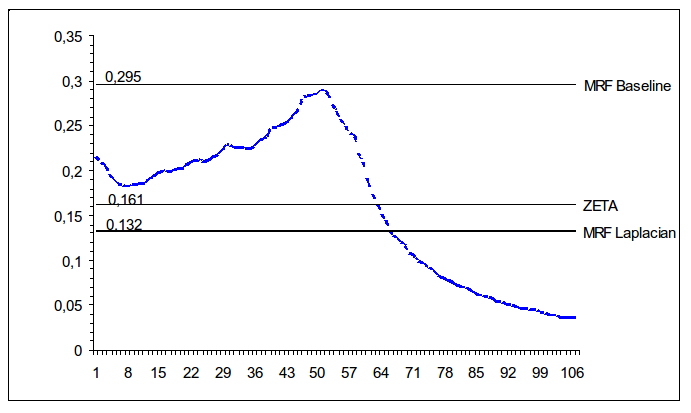
\includegraphics[width=\columnwidth]{zeta.eps}
\caption{Comparison of results from ZETA and Saxena's MRF systems. The dotted curve plots ZETA's row-wise logMAE (y-axis) as a function of the depth map row (x-axis). Full lines in the graph represent the logMAE of ZETA and Saxena's MRF for the whole hold-out set.}
\label{fig:zeta}
\end{figure}

As the graph shows, ZETA's performance is poorest around lines 30-60, which roughly corresponds to the ``middle'' of the images -- not surprisingly, this is the region where the most complex visual structures are found. ZETA's performance improves near the ``bottom'' of the images (right side of the graph), which mostly depict the ground and close-by structures. It's also noticeable that, while much more reliable than Saxena's baseline MRF system, on average ZETA does not outperform the best (Laplacian) MRF estimator. See Figure~\ref{fig:maps} for a visual comparison of depth map estimates for one image from the hold-out set.

\begin{figure}[h!]
\includegraphics[width=\columnwidth]{maps.pdf}
\caption{(a) Monocular image with natural depth information. (b) Ground truth depth. (c) Best performing MRF estimation. (d) ZETA estimation.}
\label{fig:maps}
\end{figure}

\section{Conclusion}

While current results are promising and justify further research, the present architecture clearly has its limitations. For one, the linear algorithm used for searching across bit strings is clearly inadequate at this scale, with average time for reconstructing a single depth map on the order of 10 minutes for an Intel Core 5 system. A more efficient alternative, not only in time but also space, would be a trie-based search algorithm. Tries are tree structures where each node represents a segment in a multi-dimensional key, with values stored at the leaves. Because segments are shared among different keys, each new entry added to a trie requires a little less extra space than the last; search time for the case where the exact key is present is a direct function of tree length, and approximate search can also be implemented much more efficiently. Figure~\ref{fig:trie} shows how a trie can be constructed from a list of bit strings and associated values.

\begin{figure}[h!]
\includegraphics[width=\columnwidth]{trie.pdf}
\caption{Schematic diagram of a bitwise trie storing three bit strings and associated values.}
\label{fig:trie}
\end{figure}

\begin{figure}[h!]
\includegraphics[width=\columnwidth]{dispatcher.pdf}
\caption{Alternative network assignment rule. A {\it dispatcher neuron} learns to recognize patches in terms of relative values of a vector of {\it feature histograms} and associated {\it depth estimator} neurons.}
\label{fig:dispatcher}
\end{figure}

\begin{figure}[h!]
\includegraphics[width=\columnwidth]{fourier.pdf}
\caption{An image from the spatial domain (a) is converted to its Fourier transform in the frequency domain (b). After all but 128 frequency components are zeroed (c), the inverse transform is applied, resulting in a blurred, but still largely recognizable image (d).}
\label{fig:fourier}
\end{figure}

It is also likely that the system's poor performance in the middle regions of images stems from the strategy of distributing patch / depth pairs spatially across neurons (i.e. by horizontal bands), as this prevents an object seen in one band during training to be recognized in another during testing. Instead, {\it feature histograms} could be calculated for each patch and used to train a {\it dispatcher neuron}, which would be responsible for assigning patch / depth pairs to neurons in a further layer. Figure~\ref{fig:dispatcher} illustrates the concept.

The quality of the extracted patch features should be reevaluated as well, particularly in light of new developments in neuroscience research and the physiology of vision. In recent years it has been suggested that the vertebrate eye can capture the Fourier plane of images projected onto it along with its spatial projection. This leads into the idea of sampling not patches themselves, but their Fourier transforms -- resulting in sample vectors that better capture the patches' overall structure, even if they miss the finer details. Figure~\ref{fig:fourier} illustrates the concept.

Finally, the importance of the theoretical tools introduced in this article should not be underestimated. By making explicit the capabilities as well as the limitations of the current model, they make possible to think about how VG-RAM neurons and networks could be extended with new abilities. For example, the formalization of operations on VG-RAM neurons opens the question of whether these operations themselves cannot be stored as values, and perhaps be executed is response to an access. This could in turn enable the implementation of complex calculations, inter-neuron communication protocols and multi-layer architectures.

\footnotesize

\bibliographystyle{IEEEtran}
\bibliography{references}

\normalsize

\end{document}
